%%%%%%%%%%%%%%%%%%%%%%%%%%%%%%%%%%%%%%%%%
%
% Important note:
% Chapter heading images should have a 2:1 width:height ratio,
% e.g. 920px width and 460px height.
%
%%%%%%%%%%%%%%%%%%%%%%%%%%%%%%%%%%%%%%%%%

%----------------------------------------------------------------------------------------
%	PACKAGES AND OTHER DOCUMENT CONFIGURATIONS
%----------------------------------------------------------------------------------------

\documentclass[11pt,fleqn]{book} % Default font size and left-justified equations
\usepackage{float}
\usepackage{multirow}
\usepackage{multicol}
\usepackage{parcolumns}
\usepackage{listings}

%----------------------------------------------------------------------------------------

%%%%%%%%%%%%%%%%%%%%%%%%%%%%%%%%%%%%%%%%%
% The Legrand Orange Book
% Structural Definitions File
% Version 2.0 (9/2/15)
%
% Original author:
% Mathias Legrand (legrand.mathias@gmail.com) with modifications by:
% Vel (vel@latextemplates.com)
% 
% This file has been downloaded from:
% http://www.LaTeXTemplates.com
%
% License:
% CC BY-NC-SA 3.0 (http://creativecommons.org/licenses/by-nc-sa/3.0/)
%
%%%%%%%%%%%%%%%%%%%%%%%%%%%%%%%%%%%%%%%%%

%----------------------------------------------------------------------------------------
%	VARIOUS REQUIRED PACKAGES AND CONFIGURATIONS
%----------------------------------------------------------------------------------------

\usepackage[top=3cm,bottom=3cm,left=3cm,right=3cm,headsep=10pt,a4paper]{geometry} % Page margins

\usepackage{graphicx} % Required for including pictures
\graphicspath{{Pictures/}} % Specifies the directory where pictures are stored

\usepackage{lipsum} % Inserts dummy text

\usepackage{tikz} % Required for drawing custom shapes

\usepackage[english]{babel} % English language/hyphenation

\usepackage{enumitem} % Customize lists
\setlist{nolistsep} % Reduce spacing between bullet points and numbered lists

\usepackage{booktabs} % Required for nicer horizontal rules in tables

\usepackage{xcolor} % Required for specifying colors by name
\definecolor{ocre}{RGB}{216, 67, 77} % Define the orange color used for highlighting throughout the book

%----------------------------------------------------------------------------------------
%	FONTS
%----------------------------------------------------------------------------------------

\usepackage{avant} % Use the Avantgarde font for headings
%\usepackage{times} % Use the Times font for headings
\usepackage{mathptmx} % Use the Adobe Times Roman as the default text font together with math symbols from the Sym­bol, Chancery and Com­puter Modern fonts

\usepackage{microtype} % Slightly tweak font spacing for aesthetics
\usepackage[utf8]{inputenc} % Required for including letters with accents
\usepackage[T1]{fontenc} % Use 8-bit encoding that has 256 glyphs

%----------------------------------------------------------------------------------------
%	BIBLIOGRAPHY AND INDEX
%----------------------------------------------------------------------------------------

\usepackage[style=numeric,citestyle=numeric,sorting=nyt,sortcites=true,autopunct=true,babel=hyphen,hyperref=true,abbreviate=false,backref=true,backend=biber]{biblatex}
\addbibresource{bibliography.bib} % BibTeX bibliography file
\defbibheading{bibempty}{}

\usepackage{calc} % For simpler calculation - used for spacing the index letter headings correctly
\usepackage{makeidx} % Required to make an index
\makeindex % Tells LaTeX to create the files required for indexing

%----------------------------------------------------------------------------------------
%	MAIN TABLE OF CONTENTS
%----------------------------------------------------------------------------------------

\usepackage{titletoc} % Required for manipulating the table of contents

\contentsmargin{0cm} % Removes the default margin

% Part text styling
\titlecontents{part}[0cm]
{\addvspace{20pt}\centering\large\bfseries}
{}
{}
{}

% Chapter text styling
\titlecontents{chapter}[1.25cm] % Indentation
{\addvspace{12pt}\large\sffamily\bfseries} % Spacing and font options for chapters
{\color{ocre!60}\contentslabel[\Large\thecontentslabel]{1.25cm}\color{ocre}} % Chapter number
{\color{ocre}}  
{\color{ocre!60}\normalsize\;\titlerule*[.5pc]{.}\;\thecontentspage} % Page number

% Section text styling
\titlecontents{section}[1.25cm] % Indentation
{\addvspace{3pt}\sffamily\bfseries} % Spacing and font options for sections
{\contentslabel[\thecontentslabel]{1.25cm}} % Section number
{}
{\hfill\color{black}\thecontentspage} % Page number
[]

% Subsection text styling
\titlecontents{subsection}[1.25cm] % Indentation
{\addvspace{1pt}\sffamily\small} % Spacing and font options for subsections
{\contentslabel[\thecontentslabel]{1.25cm}} % Subsection number
{}
{\ \titlerule*[.5pc]{.}\;\thecontentspage} % Page number
[]

% List of figures
\titlecontents{figure}[0em]
{\addvspace{-5pt}\sffamily}
{\thecontentslabel\hspace*{1em}}
{}
{\ \titlerule*[.5pc]{.}\;\thecontentspage}
[]

% List of tables
\titlecontents{table}[0em]
{\addvspace{-5pt}\sffamily}
{\thecontentslabel\hspace*{1em}}
{}
{\ \titlerule*[.5pc]{.}\;\thecontentspage}
[]

%----------------------------------------------------------------------------------------
%	MINI TABLE OF CONTENTS IN PART HEADS
%----------------------------------------------------------------------------------------

% Chapter text styling
\titlecontents{lchapter}[0em] % Indenting
{\addvspace{15pt}\large\sffamily\bfseries} % Spacing and font options for chapters
{\color{ocre}\contentslabel[\Large\thecontentslabel]{1.25cm}\color{ocre}} % Chapter number
{}  
{\color{ocre}\normalsize\sffamily\bfseries\;\titlerule*[.5pc]{.}\;\thecontentspage} % Page number

% Section text styling
\titlecontents{lsection}[0em] % Indenting
{\sffamily\small} % Spacing and font options for sections
{\contentslabel[\thecontentslabel]{1.25cm}} % Section number
{}
{}

% Subsection text styling
\titlecontents{lsubsection}[.5em] % Indentation
{\normalfont\footnotesize\sffamily} % Font settings
{}
{}
{}

%----------------------------------------------------------------------------------------
%	PAGE HEADERS
%----------------------------------------------------------------------------------------

\usepackage{fancyhdr} % Required for header and footer configuration

\pagestyle{fancy}
\renewcommand{\chaptermark}[1]{\markboth{\sffamily\normalsize\bfseries\chaptername\ \thechapter.\ #1}{}} % Chapter text font settings
\renewcommand{\sectionmark}[1]{\markright{\sffamily\normalsize\thesection\hspace{5pt}#1}{}} % Section text font settings
\fancyhf{} \fancyhead[LE,RO]{\sffamily\normalsize\thepage} % Font setting for the page number in the header
\fancyhead[LO]{\rightmark} % Print the nearest section name on the left side of odd pages
\fancyhead[RE]{\leftmark} % Print the current chapter name on the right side of even pages
\renewcommand{\headrulewidth}{0.5pt} % Width of the rule under the header
\addtolength{\headheight}{2.5pt} % Increase the spacing around the header slightly
\renewcommand{\footrulewidth}{0pt} % Removes the rule in the footer
\fancypagestyle{plain}{\fancyhead{}\renewcommand{\headrulewidth}{0pt}} % Style for when a plain pagestyle is specified

% Removes the header from odd empty pages at the end of chapters
\makeatletter
\renewcommand{\cleardoublepage}{
\clearpage\ifodd\c@page\else
\hbox{}
\vspace*{\fill}
\thispagestyle{empty}
\newpage
\fi}

%----------------------------------------------------------------------------------------
%	THEOREM STYLES
%----------------------------------------------------------------------------------------

\usepackage{amsmath,amsfonts,amssymb,amsthm} % For math equations, theorems, symbols, etc

\newcommand{\intoo}[2]{\mathopen{]}#1\,;#2\mathclose{[}}
\newcommand{\ud}{\mathop{\mathrm{{}d}}\mathopen{}}
\newcommand{\intff}[2]{\mathopen{[}#1\,;#2\mathclose{]}}
\newtheorem{notation}{Notation}[chapter]

% Boxed/framed environments
\newtheoremstyle{ocrenumbox}% % Theorem style name
{0pt}% Space above
{0pt}% Space below
{\normalfont}% % Body font
{}% Indent amount
{\small\bf\sffamily\color{ocre}}% % Theorem head font
{\;}% Punctuation after theorem head
{0.25em}% Space after theorem head
{\small\sffamily\color{ocre}\thmname{#1}\nobreakspace\thmnumber{\@ifnotempty{#1}{}\@upn{#2}}% Theorem text (e.g. Theorem 2.1)
\thmnote{\nobreakspace\the\thm@notefont\sffamily\bfseries\color{black}---\nobreakspace#3.}} % Optional theorem note
\renewcommand{\qedsymbol}{$\blacksquare$}% Optional qed square

\newtheoremstyle{blacknumex}% Theorem style name
{5pt}% Space above
{5pt}% Space below
{\normalfont}% Body font
{} % Indent amount
{\small\bf\sffamily}% Theorem head font
{\;}% Punctuation after theorem head
{0.25em}% Space after theorem head
{\small\sffamily{\tiny\ensuremath{\blacksquare}}\nobreakspace\thmname{#1}\nobreakspace\thmnumber{\@ifnotempty{#1}{}\@upn{#2}}% Theorem text (e.g. Theorem 2.1)
\thmnote{\nobreakspace\the\thm@notefont\sffamily\bfseries---\nobreakspace#3.}}% Optional theorem note

\newtheoremstyle{blacknumbox} % Theorem style name
{0pt}% Space above
{0pt}% Space below
{\normalfont}% Body font
{}% Indent amount
{\small\bf\sffamily}% Theorem head font
{\;}% Punctuation after theorem head
{0.25em}% Space after theorem head
{\small\sffamily\thmname{#1}\nobreakspace\thmnumber{\@ifnotempty{#1}{}\@upn{#2}}% Theorem text (e.g. Theorem 2.1)
\thmnote{\nobreakspace\the\thm@notefont\sffamily\bfseries---\nobreakspace#3.}}% Optional theorem note

% Non-boxed/non-framed environments
\newtheoremstyle{ocrenum}% % Theorem style name
{5pt}% Space above
{5pt}% Space below
{\normalfont}% % Body font
{}% Indent amount
{\small\bf\sffamily\color{ocre}}% % Theorem head font
{\;}% Punctuation after theorem head
{0.25em}% Space after theorem head
{\small\sffamily\color{ocre}\thmname{#1}\nobreakspace\thmnumber{\@ifnotempty{#1}{}\@upn{#2}}% Theorem text (e.g. Theorem 2.1)
\thmnote{\nobreakspace\the\thm@notefont\sffamily\bfseries\color{black}---\nobreakspace#3.}} % Optional theorem note
\renewcommand{\qedsymbol}{$\blacksquare$}% Optional qed square
\makeatother

% Defines the theorem text style for each type of theorem to one of the three styles above
\newcounter{dummy} 
\numberwithin{dummy}{section}
\theoremstyle{ocrenumbox}
\newtheorem{theoremeT}[dummy]{Theorem}
\newtheorem{problem}{Problem}[chapter]
\newtheorem{exerciseT}{Exercise}[chapter]
\theoremstyle{blacknumex}
\newtheorem{exampleT}{Example}[chapter]
\theoremstyle{blacknumbox}
\newtheorem{vocabulary}{Vocabulary}[chapter]
\newtheorem{definitionT}{Definition}[section]
\newtheorem{corollaryT}[dummy]{Corollary}
\theoremstyle{ocrenum}
\newtheorem{proposition}[dummy]{Proposition}

%----------------------------------------------------------------------------------------
%	DEFINITION OF COLORED BOXES
%----------------------------------------------------------------------------------------

\RequirePackage[framemethod=default]{mdframed} % Required for creating the theorem, definition, exercise and corollary boxes

% Theorem box
\newmdenv[skipabove=7pt,
skipbelow=7pt,
backgroundcolor=black!5,
linecolor=ocre,
innerleftmargin=5pt,
innerrightmargin=5pt,
innertopmargin=5pt,
leftmargin=0cm,
rightmargin=0cm,
innerbottommargin=5pt]{tBox}

% Exercise box	  
\newmdenv[skipabove=7pt,
skipbelow=7pt,
rightline=false,
leftline=true,
topline=false,
bottomline=false,
backgroundcolor=ocre!10,
linecolor=ocre,
innerleftmargin=5pt,
innerrightmargin=5pt,
innertopmargin=5pt,
innerbottommargin=5pt,
leftmargin=0cm,
rightmargin=0cm,
linewidth=4pt]{eBox}	

% Definition box
\newmdenv[skipabove=7pt,
skipbelow=7pt,
rightline=false,
leftline=true,
topline=false,
bottomline=false,
linecolor=ocre,
innerleftmargin=5pt,
innerrightmargin=5pt,
innertopmargin=0pt,
leftmargin=0cm,
rightmargin=0cm,
linewidth=4pt,
innerbottommargin=0pt]{dBox}	

% Corollary box
\newmdenv[skipabove=7pt,
skipbelow=7pt,
rightline=false,
leftline=true,
topline=false,
bottomline=false,
linecolor=gray,
backgroundcolor=black!5,
innerleftmargin=5pt,
innerrightmargin=5pt,
innertopmargin=5pt,
leftmargin=0cm,
rightmargin=0cm,
linewidth=4pt,
innerbottommargin=5pt]{cBox}

% Creates an environment for each type of theorem and assigns it a theorem text style from the "Theorem Styles" section above and a colored box from above
\newenvironment{theorem}{\begin{tBox}\begin{theoremeT}}{\end{theoremeT}\end{tBox}}
\newenvironment{exercise}{\begin{eBox}\begin{exerciseT}}{\hfill{\color{ocre}\tiny\ensuremath{\blacksquare}}\end{exerciseT}\end{eBox}}				  
\newenvironment{definition}{\begin{dBox}\begin{definitionT}}{\end{definitionT}\end{dBox}}	
\newenvironment{example}{\begin{exampleT}}{\hfill{\tiny\ensuremath{\blacksquare}}\end{exampleT}}		
\newenvironment{corollary}{\begin{cBox}\begin{corollaryT}}{\end{corollaryT}\end{cBox}}	

%----------------------------------------------------------------------------------------
%	REMARK ENVIRONMENT
%----------------------------------------------------------------------------------------

\newenvironment{remark}{\par\vspace{10pt}\small % Vertical white space above the remark and smaller font size
\begin{list}{}{
\leftmargin=35pt % Indentation on the left
\rightmargin=25pt}\item\ignorespaces % Indentation on the right
\makebox[-2.5pt]{\begin{tikzpicture}[overlay]
\node[draw=ocre!60,line width=1pt,circle,fill=ocre!25,font=\sffamily\bfseries,inner sep=2pt,outer sep=0pt] at (-15pt,0pt){\textcolor{ocre}{R}};\end{tikzpicture}} % Orange R in a circle
\advance\baselineskip -1pt}{\end{list}\vskip5pt} % Tighter line spacing and white space after remark

%----------------------------------------------------------------------------------------
%	SECTION NUMBERING IN THE MARGIN
%----------------------------------------------------------------------------------------

\makeatletter
\renewcommand{\@seccntformat}[1]{\llap{\textcolor{ocre}{\csname the#1\endcsname}\hspace{1em}}}                    
\renewcommand{\section}{\@startsection{section}{1}{\z@}
{-4ex \@plus -1ex \@minus -.4ex}
{1ex \@plus.2ex }
{\normalfont\large\sffamily\bfseries}}
\renewcommand{\subsection}{\@startsection {subsection}{2}{\z@}
{-3ex \@plus -0.1ex \@minus -.4ex}
{0.5ex \@plus.2ex }
{\normalfont\sffamily\bfseries}}
\renewcommand{\subsubsection}{\@startsection {subsubsection}{3}{\z@}
{-2ex \@plus -0.1ex \@minus -.2ex}
{.2ex \@plus.2ex }
{\normalfont\small\sffamily\bfseries}}                        
\renewcommand\paragraph{\@startsection{paragraph}{4}{\z@}
{-2ex \@plus-.2ex \@minus .2ex}
{.1ex}
{\normalfont\small\sffamily\bfseries}}

%----------------------------------------------------------------------------------------
%	PART HEADINGS
%----------------------------------------------------------------------------------------

% numbered part in the table of contents
\newcommand{\@mypartnumtocformat}[2]{%
\setlength\fboxsep{0pt}%
\noindent\colorbox{ocre!20}{\strut\parbox[c][.7cm]{\ecart}{\color{ocre!70}\Large\sffamily\bfseries\centering#1}}\hskip\esp\colorbox{ocre!40}{\strut\parbox[c][.7cm]{\linewidth-\ecart-\esp}{\Large\sffamily\centering#2}}}%
%%%%%%%%%%%%%%%%%%%%%%%%%%%%%%%%%%
% unnumbered part in the table of contents
\newcommand{\@myparttocformat}[1]{%
\setlength\fboxsep{0pt}%
\noindent\colorbox{ocre!40}{\strut\parbox[c][.7cm]{\linewidth}{\Large\sffamily\centering#1}}}%
%%%%%%%%%%%%%%%%%%%%%%%%%%%%%%%%%%
\newlength\esp
\setlength\esp{4pt}
\newlength\ecart
\setlength\ecart{1.2cm-\esp}
\newcommand{\thepartimage}{}%
\newcommand{\partimage}[1]{\renewcommand{\thepartimage}{#1}}%
\def\@part[#1]#2{%
\ifnum \c@secnumdepth >-2\relax%
\refstepcounter{part}%
\addcontentsline{toc}{part}{\texorpdfstring{\protect\@mypartnumtocformat{\thepart}{#1}}{\partname~\thepart\ ---\ #1}}
\else%
\addcontentsline{toc}{part}{\texorpdfstring{\protect\@myparttocformat{#1}}{#1}}%
\fi%
\startcontents%
\markboth{}{}%
{\thispagestyle{empty}%
\begin{tikzpicture}[remember picture,overlay]%
\node at (current page.north west){\begin{tikzpicture}[remember picture,overlay]%	
\fill[ocre!20](0cm,0cm) rectangle (\paperwidth,-\paperheight);
\node[anchor=north] at (4cm,-3.25cm){\color{ocre!40}\fontsize{220}{100}\sffamily\bfseries\thepart}; 
\node[anchor=south east] at (\paperwidth-1cm,-\paperheight+1cm){\parbox[t][][t]{8.5cm}{
\printcontents{l}{0}{\setcounter{tocdepth}{1}}%
}};
\node[anchor=north east] at (\paperwidth-1.5cm,-3.25cm){\parbox[t][][t]{15cm}{\strut\raggedleft\color{white}\fontsize{30}{30}\sffamily\bfseries#2}};
\end{tikzpicture}};
\end{tikzpicture}}%
\@endpart}
\def\@spart#1{%
\startcontents%
\phantomsection
{\thispagestyle{empty}%
\begin{tikzpicture}[remember picture,overlay]%
\node at (current page.north west){\begin{tikzpicture}[remember picture,overlay]%	
\fill[ocre!20](0cm,0cm) rectangle (\paperwidth,-\paperheight);
\node[anchor=north east] at (\paperwidth-1.5cm,-3.25cm){\parbox[t][][t]{15cm}{\strut\raggedleft\color{white}\fontsize{30}{30}\sffamily\bfseries#1}};
\end{tikzpicture}};
\end{tikzpicture}}
\addcontentsline{toc}{part}{\texorpdfstring{%
\setlength\fboxsep{0pt}%
\noindent\protect\colorbox{ocre!40}{\strut\protect\parbox[c][.7cm]{\linewidth}{\Large\sffamily\protect\centering #1\quad\mbox{}}}}{#1}}%
\@endpart}
\def\@endpart{\vfil\newpage
\if@twoside
\if@openright
\null
\thispagestyle{empty}%
\newpage
\fi
\fi
\if@tempswa
\twocolumn
\fi}

%----------------------------------------------------------------------------------------
%	CHAPTER HEADINGS
%----------------------------------------------------------------------------------------

% A switch to conditionally include a picture, implemented by  Christian Hupfer
\newif\ifusechapterimage
\usechapterimagetrue
\newcommand{\thechapterimage}{}%
\newcommand{\chapterimage}[1]{\ifusechapterimage\renewcommand{\thechapterimage}{#1}\fi}%
\newcommand{\autodot}{.}
\def\@makechapterhead#1{%
{\parindent \z@ \raggedright \normalfont
\ifnum \c@secnumdepth >\m@ne
\if@mainmatter
\begin{tikzpicture}[remember picture,overlay]
\node at (current page.north west)
{\begin{tikzpicture}[remember picture,overlay]
\node[anchor=north west,inner sep=0pt] at (0,0) {\ifusechapterimage\includegraphics[width=\paperwidth]{\thechapterimage}\fi};
\draw[anchor=west] (\Gm@lmargin,-9cm) node [line width=2pt,rounded corners=15pt,draw=ocre,fill=white,fill opacity=0.5,inner sep=15pt]{\strut\makebox[22cm]{}};
\draw[anchor=west] (\Gm@lmargin+.3cm,-9cm) node {\huge\sffamily\bfseries\color{black}\thechapter\autodot~#1\strut};
\end{tikzpicture}};
\end{tikzpicture}
\else
\begin{tikzpicture}[remember picture,overlay]
\node at (current page.north west)
{\begin{tikzpicture}[remember picture,overlay]
\node[anchor=north west,inner sep=0pt] at (0,0) {\ifusechapterimage\includegraphics[width=\paperwidth]{\thechapterimage}\fi};
\draw[anchor=west] (\Gm@lmargin,-9cm) node [line width=2pt,rounded corners=15pt,draw=ocre,fill=white,fill opacity=0.5,inner sep=15pt]{\strut\makebox[22cm]{}};
\draw[anchor=west] (\Gm@lmargin+.3cm,-9cm) node {\huge\sffamily\bfseries\color{black}#1\strut};
\end{tikzpicture}};
\end{tikzpicture}
\fi\fi\par\vspace*{270\p@}}}

%-------------------------------------------

\def\@makeschapterhead#1{%
\begin{tikzpicture}[remember picture,overlay]
\node at (current page.north west)
{\begin{tikzpicture}[remember picture,overlay]
\node[anchor=north west,inner sep=0pt] at (0,0) {\ifusechapterimage\includegraphics[width=\paperwidth]{\thechapterimage}\fi};
\draw[anchor=west] (\Gm@lmargin,-9cm) node [line width=2pt,rounded corners=15pt,draw=ocre,fill=white,fill opacity=0.5,inner sep=15pt]{\strut\makebox[22cm]{}};
\draw[anchor=west] (\Gm@lmargin+.3cm,-9cm) node {\huge\sffamily\bfseries\color{black}#1\strut};
\end{tikzpicture}};
\end{tikzpicture}
\par\vspace*{270\p@}}
\makeatother

%----------------------------------------------------------------------------------------
%	HYPERLINKS IN THE DOCUMENTS
%----------------------------------------------------------------------------------------

\usepackage{hyperref}
\hypersetup{hidelinks,backref=true,pagebackref=true,hyperindex=true,colorlinks=false,breaklinks=true,urlcolor= ocre,bookmarks=true,bookmarksopen=false,pdftitle={Title},pdfauthor={Author}}
\usepackage{bookmark}
\bookmarksetup{
open,
numbered,
addtohook={%
\ifnum\bookmarkget{level}=0 % chapter
\bookmarksetup{bold}%
\fi
\ifnum\bookmarkget{level}=-1 % part
\bookmarksetup{color=ocre,bold}%
\fi
}
}

\begin{document}

%----------------------------------------------------------------------------------------
%	TITLE PAGE
%----------------------------------------------------------------------------------------

\begingroup
\thispagestyle{empty}
\begin{tikzpicture}[remember picture,overlay]
\node[inner sep=0pt] (background) at (current page.center) {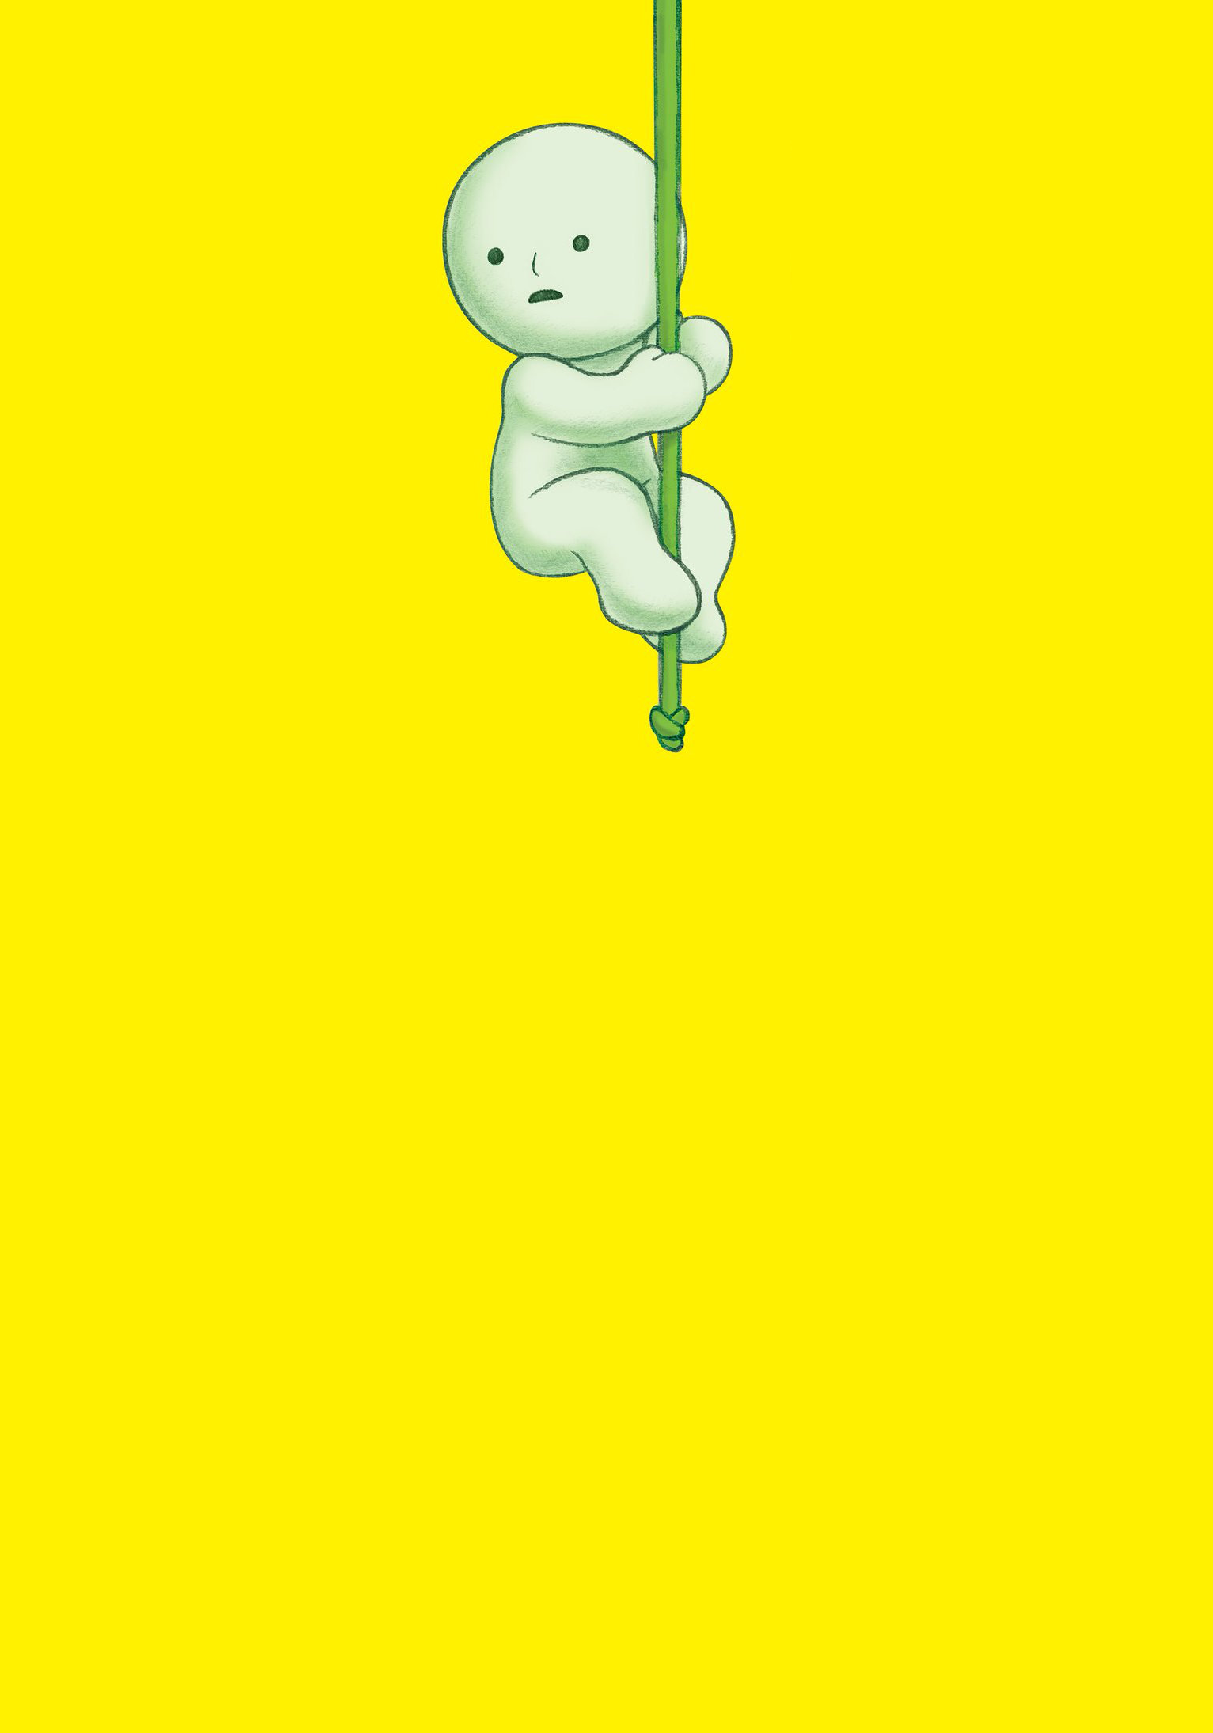
\includegraphics[width=\paperwidth]{background}};
\draw (current page.center) node [fill=white,fill opacity=0.6,text opacity=1,inner sep=1cm]{\Huge\centering\bfseries\sffamily\parbox[c][][t]{\paperwidth}{\centering Machine Learning and Optimisation\\[15pt]
{\Large COMP24111 Course Notes}\\[20pt]
{\huge Jonathan Tang}}};
\end{tikzpicture}
\vfill
\endgroup

%----------------------------------------------------------------------------------------
%	COPYRIGHT PAGE
%----------------------------------------------------------------------------------------

\newpage
~\vfill
\thispagestyle{empty}

\noindent Copyright \copyright\ 2017 Jonathan Tang\\

\noindent \textbf{jtang0506.github.io}

%----------------------------------------------------------------------------------------
%	TABLE OF CONTENTS
%----------------------------------------------------------------------------------------

%\usechapterimagefalse % If you don't want to include a chapter image, use this to toggle images off - it can be enabled later with \usechapterimagetrue

\chapterimage{chapter_head_1.pdf} % Table of contents heading image

\pagestyle{empty} % No headers

\tableofcontents % Print the table of contents itself

\cleardoublepage % Forces the first chapter to start on an odd page so it's on the right

\pagestyle{fancy} % Print headers again

%----------------------------------------------------------------------------------------
%	PART 1
%----------------------------------------------------------------------------------------

\part{Section I}

%----------------------------------------------------------------------------------------
%	Introduction to Machine Learning
%----------------------------------------------------------------------------------------

\chapterimage{chapter_head_2.pdf}

\chapter{Introduction to Machine Learning}

\section{Supervised learning}\index{supervised learning}
In \textbf{supervised learning} problems, there is an input, $X$, an target output, $Y$, provided by a \textit{teacher} and the task is to learn the relationship between the input and the output. A training example in supervised learning is the pair ($x$, $y$) where $x$ is the input and $y$ is the target output. The labels provided with the training samples are know as the \textbf{ground truth}\index{ground truth}. We assume a model defined up to a set of parameters, $y = g(x \, \vert \, \theta)$ where $g(\cdot)$ is the model and $\theta$ are its parameters.
\subsection{Classification}
For a classification\index{supervised learning!classification} problem, the task of the classifier is to assign a class label to a given input. For example, a classification problem may be to decide whether an image contains a picture of a cat or a dog, or neither.

\subsection{Regression}
Suppose we want to predict the salary of a Computer Science graduate role. Inputs are the students attributes - that we believe affects a graduate's worth. The output is the predicted salary. Such problems where the output is a continuous number is known as a \textbf{regression}\index{Supervised learning!regression} problem.

\section{Unsupervised learning}\index{unsupervised learning}
Unlike in supervised learning, we do not have a supervisor and we only have input data. The task in \textbf{unsupervised learning} is to form a natural understanding of the hidden structure of unlabelled data. There is a structure to the input space such that certain patterns occur more often than others, and we want to see what generally happens and what does not.

\section{Reinforcement learning}\index{reinforcement learning}
In reinforcement learning, there is a \textit{teacher} who provides feedback on the action of an agent, in terms of reward and punishment.
%----------------------------------------------------------------------------------------
%	k-Nearest Neighbour
%----------------------------------------------------------------------------------------

\chapterimage{chapter_head_2.pdf}

\chapter{k-nearest Neighbour}\index{k-nearest Neighbour}
The \textbf{k-nearest Neighbour} estimation is one of the simplest machine learning algorithms, it is a \textbf{non-parametric method} (no parameter needs to be optimised) and requires \textbf{no explicit training}.

\section{k-nearest Neighbour Classification}\index{k-nearest Neighbour!classification}
The \textit{k}-nearest neighbour classifier assigns an instance to the class most heavily represented among its \textit{k} neighbours. It is based on the idea that the more similar the instances, the more likely it is that they belong to the same class. We measure how similar two data points are by using a reasonable similarity or distance measure.

\subsection{k-NN classification rule}
\begin{lstlisting}[mathescape]
let $x_{te}$ be the testing point
for each training data point $x_{tr}$
    measure distance($x_{te}$, $x_{tr}$)
end
sort distances
select $k$ nearest points
assign most common class to $x_{te}$	
\end{lstlisting}

\noindent
In order to measure the distance $d(x_{te}, x_{tr})$ mentioned in the algorithm, we need to first decide on a distance measure. Euclidean distance and inner product are two measures we can used, that are defined below. An additional distance measure that we can use is cosine similarity, which is described in a later chapter.\\

\begin{exercise}
The hyper-parameter $k$ should be odd and co-prime to the number of classes in the data set, why?
\end{exercise}

\begin{definition}[Euclidean Distance]
Given two $d$-dimensional data points, $\mathbf{p}$ and $\mathbf{q}$, where $\mathbf{p}= \big[p_1, p_2, \cdots, p_d\big]$ and $\mathbf{q} = \big[q_1, q_2, \cdots, q_d\big]$, we define the \textbf{Euclidean distance}\index{similarity / distance measures!Euclidean distance} $d(\mathbf{p},\mathbf{q})$ as:
\begin{equation*}
	d(\mathbf{p},\mathbf{q}) \, = \, \sqrt{(p_1 - q_1)^2 + (p_2 - q_2)^2 + \cdots + (p_d - q_d)^2} \, = \, \sqrt{\sum^d_{i=1}(p_i - q_i)^2}
\end{equation*}
In this case, the \textit{k}-nearest neighbours are the training points with the lowest Euclidean distances to the testing point.
\end{definition}

\begin{definition}[Inner Product]
Given two $d$-dimensional data points, $\mathbf{p}$ and $\mathbf{q}$, where $\mathbf{p}= \big[p_1, p_2, \cdots, p_d\big]$ and $\mathbf{q} = \big[q_1, q_2, \cdots, q_d\big]$, we define the \textbf{inner product}\index{similarity / distance measures!inner product} as:
\begin{equation*}
	s_{inner}(\mathbf{p},\mathbf{q}) \, = \, \sum^d_{i=1}p_iq_i
\end{equation*}
Since the inner product is a similarity measure, the \textit{k}-nearest neighbours are the training points possessing the highest similarity values to the testing point.
\end{definition}

\section{k-Nearest Neighbour Regression}\index{k-nearest Neighbour!regression}
For regression, we take a sample's $k$ nearest neighbours to estimate its target output, for example, through the weighted average of these neighbours target output. This is very similar to classification but you need to take into account the distance of this sample from its nearest neighbours.

\subsection*{Worked Example}
Since the $k$-NN classification algorithm is one of the simplest, you should be able to follow it from the lecture slides - hence a worked example has been omitted. It is also trivial to derive the algorithm for k-NN regression.

\section{Neighbour number $k$}
The neighbour number $k$ is called the \textbf{hyper-parameter}\index{hyper-parameter} and the processing of determining the best value of $k$ to use is called \textbf{hyper-parameter selection}\index{hyper-parameter selection} or model selection. If our choice of $k$ is too small, we may model noise and if our choice of $k$ is too large, neighbours will include too many samples from other classes.\\

\noindent
The number of training samples also plays a role, a small number of training samples will lead to insufficient information about the data set. However, a large number of training samples comes with a tradeoff in time and memory cost for calculating and sorting distances.

%----------------------------------------------------------------------------------------
%	Linear Classification and Regression
%----------------------------------------------------------------------------------------

\chapterimage{chapter_head_2.pdf}

\chapter{Linear Classification and Regression}

%----------------------------------------------------------------------------------------
%	Logistic Regression
%----------------------------------------------------------------------------------------

\chapterimage{chapter_head_2.pdf}

\chapter{Logistic Regression}

%----------------------------------------------------------------------------------------
%	Support Vector Machine
%----------------------------------------------------------------------------------------

\chapterimage{chapter_head_2.pdf}

\chapter{Support Vector Machine}

\section{Model Validation}\index{model validation}
\subsection{Holdout method}\index{model validation!holdout method}
With the \textbf{holdout method}, the whole dataset is split into two groups, a training set and a testing set. The model is trained using the training set and asked to predict output values for the data in the testing set, which it has never seen before. This evaluation can have a high variance as we may get an unfortunate split as it may depend heavily on which data points end up in the training set and which end up in the testing set. Another drawback is that we may only have a small dataset, so we may not afford to set aside a portion of the dataset for testing.

\subsection{Random subsampling}
% TODO: Random Subsampling

\subsection{k-fold cross validation}\index{model validation!k-fold cross validation}
\textbf{k-fold cross validation} is one way to improve over the holdout method, the dataset is divided into $k$ partitions and the holdout method is performed $k$ times. Each time, one of the $k$ subsets is used as the testing set and the remaining $k - 1$ subsets are combined and used as the training set. We evaluate the error estimate as the average error across the $k$ trials. The advantage of this method is that it matters less how the dataset gets divided and all the examples in the dataset are eventually used for both training and testing, therefore the variance of the resulting estimate is reduced as $k$ is increased. However, the training has to be done $k$ times, which means this method gets expensive to compute as $k$ is increased.

\subsection{Leave-one-out cross validation}\index{model validation!LOO cross validation}
\textbf{Leave-one-out cross validation} is the degenerate case for $k$-fold cross validation, with $k$ = $N$, the number of data points in the dataset. As before, the average error is computed and used to evaluate the model. The evaluation given by leave-one-out cross validation error is good, but it is very expensive to compute compared to other methods.

\subsection{Bootstrap}
% TODO: Bootstrap

\section{Confusion matrix}\index{confusion matrix}
A confusion matrix is a table with two rows and two columns which allows further analysis rather than just the proportion of correct classifications. For example, if we had a dataset containing 98 examples from Class 1 and 2 examples from Class 2, there may be a classifier which classifies all the observations as Class 1, which yields a overall accuracy of 98\%. However, accuracy is not a reliable metric for this classifier as the classifier would have 100\% recognition rate for Class 1 but 0\% recognition rate for Class 2.\\

\begin{definition}[True Positives (TP)]\index{confusion matrix!true positive}
Both the predicted class and actual class is 'Yes'.
\end{definition}
\begin{definition}[True Negatives (TN)]\index{confusion matrix!true negative}
Both the predicted class and actual class is 'No'.
\end{definition}
\begin{definition}[False Positives (FP)]\index{confusion matrix!false positive}
The predicted class is 'Yes' and actual class is 'No'.
\end{definition}
\begin{definition}[False Negatives (FN)]\index{confusion matrix!false negative}
The predicted class is 'No' and actual class is 'Yes'.
\end{definition}

\subsection*{Worked Example}
Suppose that we predicted the presence of a disease that a patient and obtain the results below.
\begin{table}[h]
\centering
\begin{tabular}{c|c|cc}
\multicolumn{2}{c|}{\multirow{2}{*}{n = 165}} & \multicolumn{2}{c}{Predicted Class} \\ \cline{3-4} 
\multicolumn{2}{c|}{} & No & Yes \\ \hline
\multirow{2}{*}{\begin{tabular}[c]{@{}c@{}}Actual\\ Class\end{tabular}} & No & 50 & 10 \\
 & Yes & 5 & 100
\end{tabular}
\end{table}

\begin{example}
	For the above example, \textbf{TP} = 100, \textbf{TN} = 50, \textbf{FP} = 10 and \textbf{FN} = 5.
\end{example}

\noindent
Some questions we may want to ask about our predictions are:
\begin{enumerate}
	\item When the patient actually has the disease, how often did we predict this?
	\item When the patient does not have the disease, how often did we predict this?
	\item When we predict that a patient has a disease, how often are we correct?
\end{enumerate}

\noindent
\\First, we define some terms which directly relate to the questions above.\\

\begin{definition}[Sensitivity / Recall]\index{confusion matrix!sensitivity}\index{confusion matrix!recall}
The proportion of positives that are correctly classified.
\begin{equation*}
	\frac{\text{True Positives}}{\text{Number of Actual Positives}} = \frac{\text{TP}}{\text{TP+FN}}
\end{equation*}
\end{definition}

\begin{definition}[Specificity]\index{confusion matrix!specificity}
The proportion of negatives that are correctly classified.
\begin{equation*}
	\frac{\text{True Negatives}}{\text{Number of Actual Negatives}} = \frac{\text{TN}}{\text{TN+FP}}
\end{equation*}
\end{definition}

\begin{definition}[Precision]\index{confusion matrix!precision}
The proportion of predicted positives which were positive.
\begin{equation*}
	\frac{\text{True Positives}}{\text{Number of Predicted Positives}} = \frac{\text{TP}}{\text{TP+FP}}
\end{equation*}
\end{definition}

\begin{example}
	By definition, the answers to the above questions are sensitivity, specificity and precision respectively.
\end{example}

\begin{exercise}
Calculate the sensitivity, specificity and precision for the confusion matrix given above.
\end{exercise}

%----------------------------------------------------------------------------------------
%	Deep Learning Models
%----------------------------------------------------------------------------------------

\chapterimage{chapter_head_2.pdf}

\chapter{Deep Learning Models}

%----------------------------------------------------------------------------------------
%	PART 2
%----------------------------------------------------------------------------------------

\part{Section II}

%----------------------------------------------------------------------------------------
%	Generative Models and Naive Bayes
%----------------------------------------------------------------------------------------

\chapterimage{chapter_head_2.pdf}

\chapter{Generative Models and Naive Bayes}

%----------------------------------------------------------------------------------------
%	Clustering Analysis Basics
%----------------------------------------------------------------------------------------

\chapterimage{chapter_head_2.pdf}

\chapter{Clustering Analysis Basics}

\section*{Introduction}
Clustering analysis is the process of finding similarities between data according to the characteristics underlying he data and grouping similar data objects into clusters. A \textbf{cluster}\index{cluster} is a group of data points which are similar to one another within the same group and dissimilar to the points in other groups. Clustering analysis is \textbf{unsupervised} as there are no predefined classes for a training data set. The main approach of clustering analysis is to maximise the intra-cluster similarity and minimise the inter-cluster similarity. Typically, clustering analysis is either used as a stand-alone tool to gain an insight into data distribution or used as a preprocessing step of other algorithms in intelligent systems.\\

\noindent
The two general tasks of clustering analysis are:
\begin{enumerate}
	\item Identifying the "natural" number of clusters present in a data set
	\item Properly grouping data points into "sensible" clusters
\end{enumerate}

\subsection*{Real Life Applications}
\begin{itemize}
	\item \textbf{Marketing} - companies can discover distinct groups in their customer bases and then use this knowledge to develop targeted marketing programs
	\item \textbf{Social network mining} - discovering communities of similar interests in a large group of people
	\item \textbf{Image segmentation} - dividing an image into distinct regions for object recognition
\end{itemize}

\section{Data Representation}\index{data representation}
\begin{multicols}{2}
\noindent
A data matrix is a $n \times p$ matrix which represents $n$ data points with $p$ dimensions. The data matrix has $two$ modes as rows and columns represent different entities.
\columnbreak
\begin{equation*}
	\begin{bmatrix}
		x_{11} & x_{12} & \cdots & x_{1p} \\
		x_{21} & x_{22} & \cdots & x_{2p} \\
		\vdots & \vdots & \vdots & \vdots \\
		x_{n1} & x_{n2} & \cdots & x_{np} \\
	\end{bmatrix}
\end{equation*}
\end{multicols}

\begin{multicols}{2}
\noindent
A distance / dissimilarity matrix is a $n \times n$ matrix which represents the distance between each data point. The distance matrix is a symmetric triangular matrix as $\mathbf{d}(x, y) = \mathbf{d}(y, x)$ where $x, y$ are two data points. The distance matrix has $one$ mode as the rows and column represent the distance for the same entity.
\columnbreak
\begin{equation*}
	\begin{bmatrix}
		0 & & & & \\
		d(x_2, x_1) & 0 & & & \\
		d(x_3, x_1) & d(x_3, x_2) & 0 & & \\
		\vdots & \vdots & \vdots & \ddots & \\
		d(x_n, x_1) & d(x_n, x_2) & d(x_n, x_3) & \cdots & 0\\
	\end{bmatrix}
\end{equation*}
\end{multicols}

\section{Distance Measures}\index{distance measures}
The \textbf{Minkowski distance} is a metric in a normed vector space which can be considered as the generalisation of both the Euclidean distance and the Manhattan distance. \\

\begin{definition}[Minkowski Distance]\index{distance measures!Minkowski distance}
The Minkowski distance of order $p$ between two points $\mathbf{x} = (x_1, x_2, \cdots, x_n)$ and $\mathbf{y} = (y_1, y_2, \cdots, y_n)$ is defined as:
\begin{equation*}
	d(\mathbf{p},\mathbf{q}) \, = \, \Bigg(\vert x_1 - y_1 \vert^p + \vert x_2 - y_2 \vert^p + \cdots + \vert x_n - y_n \vert^p \Bigg)^{\frac{1}{p}}, p > 0
\end{equation*}
\end{definition}

\noindent
The value of $p$ in the Minkowski Distance would be selected depending on the application. The \textbf{Manhattan} and \textbf{Euclidean} distances are simply Minkowski distances of order 1 and 2 respectively.\\

\begin{definition}[Manhattan Distance]\index{distance measures!Manhattan distance}
\begin{equation*}
	d(\mathbf{p},\mathbf{q}) \, = \, \vert x_1 - y_1 \vert + \vert x_2 - y_2 \vert + \cdots + \vert x_n - y_n \vert
\end{equation*}
This is also known as the city block distance, the reason becomes clear in the examples below.
\end{definition}

\begin{definition}[Euclidean Distance]\index{distance measures!Euclidean distance}
\begin{equation*}
	d(\mathbf{p},\mathbf{q}) \, = \, \sqrt{\vert x_1 - y_1 \vert^2 + \vert x_2 - y_2 \vert^2 + \cdots + \vert x_n - y_n \vert^2}
\end{equation*}
This is the distance that you are already familiar with, in $n$ dimensions.
\end{definition}

\begin{exercise}
When is the Manhattan distance between $x$ and $y$ equal to the Euclidean distance between $x$ and $y$, where $x$ and $y$ are data points of two dimensions?
\end{exercise}

\begin{definition}[Cosine measure]\index{distance measures!Cosine measure}
For $\mathbf{x} = (x_1, x_2, \cdots, x_n)$ and $\mathbf{y} = (y_1, y_2, \cdots, y_n)$
\begin{equation*}
	\cos(\mathbf{x}, \mathbf{y}) = \frac{x_1y_1 + \cdots + x_ny_n}{\sqrt{x_1^2 + \cdots + x_n^2} \; \sqrt{y_1^2 + \cdots + y_n^2}} \quad \text{and} \quad d(\mathbf{x}, \mathbf{y}) = 1 - \cos(\mathbf{x}, \mathbf{y})
\end{equation*}
Note that $-1 \leq \cos(\mathbf{x}, \mathbf{y}) \leq 1$ and $0 \leq d(\mathbf{x}, \mathbf{y}) \leq 2$
\end{definition}

\newpage

\subsection*{Worked Example}
Suppose we have some documents that we want to compare to see how similar texts are, without taking into account the order of the words. For this example, we will consider:\\

\begin{enumerate}[label=(\alph*)]
	\item Labeeba loves me more than Hani loves me
	\item Hani loves Labeeba more than Labeeba loves Hani
	\item Labeeba likes Hani more than Hani likes Labeeba
\end{enumerate}

\ \\ \noindent
First, we make a list of all the words that appear across all texts.
\begin{center}
	[Hani, Labeeba, likes, loves, me, more, than]
\end{center}

\noindent
Next, we construct a vector for each document, with the frequency of each word.
\begin{center}
	\textbf{a} = [1, 1, 0, 2, 2, 1, 1]\\
	\textbf{b} = [2, 2, 0, 2, 0, 1, 1]\\
	\textbf{c} = [2, 2, 2, 0, 0, 1, 1]\\
\end{center}

\noindent
Now we can compute the \textbf{cosine measures}: cos(\textbf{a}, \textbf{b}), cos(\textbf{a}, \textbf{c}) and cos(\textbf{b}, \textbf{c}).

\begin{equation*}
	\cos(\mathbf{a}, \mathbf{b}) = \frac{(1)(1) + (1)(2) + (0)(0) + (2)(2) + (2)(0) + (1)(1) + (1)(1)}{\sqrt{1^2 + 1^2 + 0^2 + 2^2 + 2^2 + 1^2 + 1^2} \, \sqrt{2^2 + 2^2 + 0^2 + 2^2 + 0^2 + 1^2 + 1^2}} \approx 0.694
\end{equation*}

\noindent
By similar calculations, we find that $\cos(\mathbf{a}, \mathbf{c}) \approx 0.463$ and $\cos(\mathbf{b}, \mathbf{c}) \approx 0.714$. This tells us that sentences \textbf{b} and \textbf{c} are the most similar pair out the above texts, as they have the highest cosine measure. This is also the reason $d(\mathbf{x}, \mathbf{y})$ is defined as $1 - \cos(\mathbf{x}, \mathbf{y})$ since a larger cosine measure would be converted into a smaller distance.

\section{Distance for binary features}\index{binary features!distance}
For binary features, their values can be converted to 1 or 0, then we calculate the contingency table.\index{binary features!contingency table}

\begin{table}[h]
\centering
\begin{tabular}{cccc}
\multicolumn{2}{c}{\multirow{2}{*}{}}       & \multicolumn{2}{c}{y} \\
\multicolumn{2}{c}{}                        & 1         & 0         \\ \cline{2-4} 
\multirow{2}{*}{x} & \multicolumn{1}{c|}{1} & a         & b         \\
                   & \multicolumn{1}{c|}{0} & c         & d        
\end{tabular}
\end{table}

\subsection*{Symmetric binary features}\index{binary features!symmetric}
Binary features are \textbf{symmetric} if both of their states equally valuable and carry the same weight; i.e. no
preference on which outcome should be coded as 1 or 0 , e.g. gender.

\begin{center}
	$$d(\mathbf{x}, \mathbf{y}) = \frac{b + c}{a + b + c + d}$$
\end{center}


\subsection*{Asymmetric binary features}\index{binary features!asymmetric}
Binary features are \textbf{asymmetric} if the outcomes of the states not equally important, e.g. the positive and negative
outcomes of a disease test; the rarest one is set to 1 and the other is 0. Since the number of negative matches are considered unimportant, they are omitted from the calculations.

\begin{center}
	$$d(\mathbf{x}, \mathbf{y}) = \frac{b + c}{a + b + c}$$
\end{center}

\section{Distance for nominal features}\index{nominal features!distance}
Nominal features are those that can take more than two states, for example {\textit{small, medium, large}}. There are two methods to handle variables with nominal features; simple mis-matching and converting them into binary variables.

\subsection*{Simple mis-matching}\index{nominal features!simple mismatching}
$$d(\mathbf{x}, \mathbf{y}) = \frac{\text{number of mis-matching features between \textbf{x} and \textbf{y}}}{\text{total number of features}}$$

\subsection*{Converting them into binary variables}\index{nominal features!converting into binary}
We create new binary features for all of its nominal states, for example if our size feature takes three possible nominal states \textit{{small, medium, large}} then this feature will be expanded into three binary features. \textit{{small, medium, large}} = {100, 010, 001}, then we can use the distance measures for binary features.

\subsection*{Worked Example}
Consider the example below where we have two toys, $T_1$ and $T_2$, whose features are size, colour and price range.
\begin{table}[h]
\centering
\begin{tabular}{c|c|c|c|}
\cline{2-4}
                         & Size & Colour & Price Range \\ \hline
\multicolumn{1}{|c|}{$T_1$} & 010  & 100    & 01       \\ \hline
\multicolumn{1}{|c|}{$T_2$} & 100  & 001    & 01      \\ \hline
\end{tabular}
\end{table}

\subsubsection*{Simple mis-matching}
Only the price range takes the same value for the features between $T_1$ and $T_2$ hence
$$d(\mathbf{T_1}, \mathbf{T_2}) = \frac{2}{3} \approx 0.66$$

\subsubsection*{Converting them into binary values}
Size: [Small, Medium, Large] = [100, 010, 000]\\
Colour: [Green, Red, Yellow] = [100, 010, 000]\\
Price: [Cheap, Expensive] = [10, 01]\\

\noindent
Now we do $T_1$ \textbf{XOR} $T_2$ = 01010001 \textbf{XOR} 10000101 = 11010100. Now from here we can get the distance by dividing the number of 1 bits in $T_1$ \textbf{XOR} $T_2$ by the total number of bits in $T_1$.
$$d(\mathbf{T_1}, \mathbf{T_2}) = \frac{4}{8} = 0.5$$

\section{Clustering methodologies}\index{clustering methodologies}
\begin{itemize}
	\item \textbf{Partitioning}: construct various partitions and then evaluate them by some criterion, e.g. minimising the sum of squares distance cost
	\item \textbf{Hierarchical}: create a hierarchical decomposition of the set of data using some criterion
	\item \textbf{Density-based}: based on connectivity and density functions
	\item Model-based: a generative model is hypothesised for each of the clusters and tries to find the best fir of that model to each other
	\item \textbf{Spectral clustering}: convert data set into a weighted graph then cut the graphs into sub-graphs corresponding to clusters via spectral analysis
	\item \textbf{Clustering ensemble}: combine multiple clustering results
\end{itemize}

%----------------------------------------------------------------------------------------
%	k-means Clustering
%----------------------------------------------------------------------------------------

\chapterimage{chapter_head_2.pdf}

\chapter{k-means Clustering}

\section*{Introduction}
The k-means algorithm is the simplest partitioning method for clustering analysis and is widely used in data mining algorithms. It is a \textbf{heuristic method} and is based on each clustering being represented by the centre of the cluster and the algorithm will converge to stable centroids\index{centroid} of clusters. The goal of this algorithm is find a partition of $k$ clusters to optimise the chosen partition criterion - the global optimum is achieved by exhaustively searching all partitions.

\section{Partitioning clustering approach}\index{partitioning clustering}
A partitioning clustering approach is done by iteratively partitioning the training data set to learn a partition of the given data space to product several non-empty clusters, where the number of clusters is usually given in advance. In principle, an optimal partition is achieved by minimising the sum of the squared distance to its "representative object" in each cluster.

\begin{exercise}
Why do we have to used the squared distance?
\end{exercise}

\section{k-means algorithm}
Before we can use the k-means algorithm, we must decide the cluster number \textit{k} and an appropriate distance measure that will be used. We initialise the algorithm by selecting \textit{k} distinct seed points, randomly.\\

\begin{enumerate}
	\item assign each object to the cluster of the nearest point
	\item compute new seed points as the centroids of the clusters of the current partition
\end{enumerate}

\ \\ \noindent
The two steps are repeated until it converges (membership in each cluster no longer changes). At this point, we have \textit{k} centroids which partition the whole data space into \textit{k} mutually exclusive subspaces to form a partition.\\

\begin{figure}[h]
	\centering
  	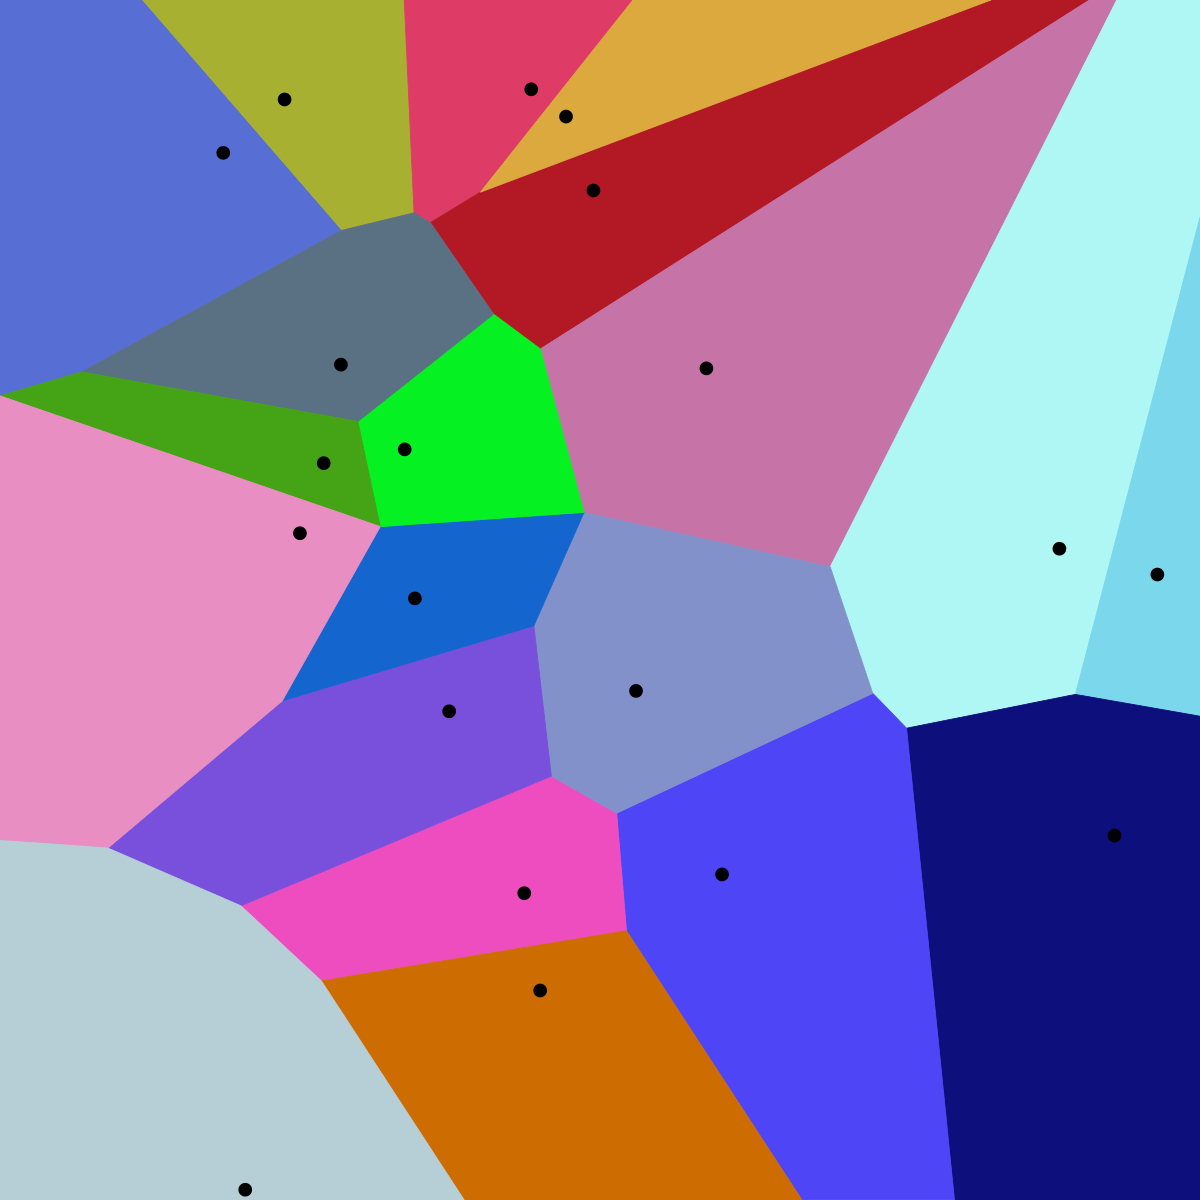
\includegraphics[width=50mm, scale=0.7]{Pictures/voronoi}
  	\caption{Voronoi Diagram}
\end{figure}

\noindent
The figure above shows how a data space can be partitioned, where each black dot represents a centroid of a cluster. Notice that the distance used above is Euclidean distance.

\section{Issues}

\begin{itemize}
	\item This algorithm has computational complexity of \textit{O}(tKn), where \textit{n} is the number of data points, \textit{K} is the number of clusters and \textit{t} is the number of iterations. Normally, \textit{K}, \textit{t} << \textit{n}.
	\item It is sensitive to initialisation, which may result to unwanted solutions
	\item Is unable to handle noisy data and outliers, which results in an inaccurate partition
	\item Requires prior knowledge of the cluster number
	\item Incapable of handling clusters of non-convex shape
	\item Inapplicable to categorical data, since the mean is not defined
	\item How do we evaluate the k-mean performance? 
\end{itemize}

\subsection*{Example}
The k-Means algorithm is very simple, so an example has be omitted. An example may be added in the future, if I have spare time - but for now, just check the lecture slides.

%----------------------------------------------------------------------------------------
%	Hierarchical and Ensemble Clustering
%----------------------------------------------------------------------------------------

\chapterimage{chapter_head_2.pdf}

\chapter{Hierarchical and Ensemble Clustering}

\section{Hierarchical clustering approach}
Hierarchical clustering approach\index{hierarchical clustering} is done by sequentially partitioning the data set to construct nested partitions layer by layer, via grouping objects into a tree of clusters. We use a generalised distance matrix as the clustering criteria and we do not need to know the number of clusters in advance.

\subsection*{Approaches to hierarchical clustering}\index{hierarchical clustering!approaches}
There are two main approaches to hierarchical clustering: \textbf{agglomerative clustering}\index{hierarchical clustering!agglomerative} (bottom-up) and \textbf{divisive clustering}\index{hierarchical clustering!divisive} (top-down). In agglomerative clustering, each data point is initially its own atomic cluster and we merge clusters into larger and larger clusters. Divisive clustering, as the name suggests, is where all data points belong to a single cluster initially, then the cluster is divided into smaller and smaller clusters.

\section{Cluster distance measures}\index{cluster distance measures}
\ 
\begin{definition}[Single link]\index{cluster distance measures!single link}
	The \textbf{smallest} distance between an element in one cluster and an element in another, i.e. $d(C_i, C_j) = \text{min}\{d(x_{ip}, x_{jq})\}$ 
\end{definition}

\begin{definition}[Complete link]\index{cluster distance measures!complete link}
	The \textbf{largest} distance between an element in one cluster and an element in another, i.e. $d(C_i, C_j) = \text{max}\{d(x_{ip}, x_{jq})\}$ 
\end{definition}

\begin{definition}[Average]\index{cluster distance measures!average}
	The \textbf{average} distance between elements in one cluster and elements in the other, i.e. $d(C_i, C_j) = \text{avg}\{d(x_{ip}, x_{jq})\}$ 
\end{definition}

\newpage
\section{Agglomerative clustering}
\subsection*{Algorithm}
\begin{enumerate}
	\item Select a cluster distance measure to use
	\item Convert all object features into a distance matrix
	\item Set each object as an atomic cluster (N objects means N clusters at start)
	\item Repeat until number of clusters is one (or known \# of clusters)
	\begin{itemize}
		\item Merge two closest clusters
		\item Update distance matrix
	\end{itemize}
\end{enumerate}

\subsection*{Example}
Again, very simple algorithm - so an example has been omitted as the lecture example is sufficient.\\

\begin{definition}[Lifetime]\index{lifetime}
	The distance between that a cluster is created and that it disappears (merges with other clusters during clustering).
\end{definition}

\begin{definition}[k-cluster lifetime]\index{k-cluster lifetime}
	The distance from that $K$ clusters emerge to that $K$ clusters vanish (due to the reduction to $K-1$ clusters).
\end{definition}

\section*{Relevant Issues}
\begin{itemize}
	\item How do we determine the number of clusters?
	\begin{itemize}
		\item If the number of clusters is known, then we have a termination condition
		\item We can use the \textbf{K-cluster lifetime} as a range of threshold values on the dendrogram that leads to the identification of $K$ clusters
		\item Heuristic method: cut the dendrogram tree with maximum life time to find a "proper" $K$
		\end{itemize}
	\item Major weakness of agglomerative clustering methods
	\begin{itemize}
		\item Can never undo what was done previously...
		\item Sensitive to cluster distance measures, noise and outliers
		\item Efficiency of $O(n^2\log n)$, where $n$ is the number of total objects
	\end{itemize}
\end{itemize}

\section{Ensemble Clustering}\index{ensemble clustering}
\textbf{Ensemble clustering} is concerned with the issues that may affect a single clustering algorithm, for example, sensitivity to initialisation, noise, outliers, distance metrics and it may be hard to choose a single algorithm which can handle all types of cluster shapes and sizes. The purpose of ensemble clustering is to utilise the results obtained by multiple clustering analyses for robustness.

\subsection*{Algorithm summary}
\begin{enumerate}
	\item Perform clustering analysis by using either different clustering algorithms or running a single clustering algorithm of different conditions, \textbf{leading to multiple partitions}
	\item Convert clustering results on different partitions into \textbf{binary distance measure}
	\item Evidence accumulation: form a \textbf{collective distance matrix} based on all the distance matrices
	\item Apply a hierarchical clustering algorithm (with a proper cluster distance measure) to collective distance matrix and \textbf{use the maximum $k$-cluster lifetime to decide}
\end{enumerate}

%----------------------------------------------------------------------------------------
%	Cluster Validation
%----------------------------------------------------------------------------------------

\chapterimage{chapter_head_2.pdf}

\chapter{Cluster Validation}
\section*{Introduction}
Cluster validation refers to the procedures that evaluate the results of clustering in a \textit{quantitive} and \textit{objective} fashion. In cluster validation, we need to compare clustering algorithms, solve the problem of determining the number of clusters, avoid finding patterns in noise and finding the "best" clusters from the data.\\

\noindent
We have two types of criteria, internal and external. An \textbf{internal criteria}\index{internal index} (index) is used to validate without external information and can be applied to find the "proper" number of clusters in a data set. An \textbf{external criteria}\index{external index} (index) may be applied to evaluate the performance of a clustering algorithm against data sets where the ground truth is available, by comparing how similar the partition generated by the clustering algorithm is to the ground truth.

\section{Internal Index}
The internal index we will focus on is the \textbf{F-ratio index}, which is a variance based internal index.

\subsection*{Variance-based methods}
In \textbf{variance-based methods}\index{variance-based methods}, the goal is to minimise the intra-cluster variance and to maximise the inter-cluster variance. Assume an algorithm leads to a partition of $K$ clusters where cluster $i$ has $n_i$ data points, $c_i$ is its centroid and $d(\cdot,\cdot)$ is a chosen distance measure.

$$ \text{Intra-cluster variance = } SSW(K) = \sum^K_{i=1}\sum^{n_i}_{j=1}d^2(\mathbf{x}_{ij}, \mathbf{c}_i)$$
$$ \text{Inter-cluster variance = } SSB(K) = \sum^K_{i=1}n_i \cdot d^2(\mathbf{c}_i, \mathbf{c})$$
$$ \text{where \textbf{c} is the global centroid of the whole data set} $$

\subsection{F-ratio index}
The \textbf{F-ratio index}\index{F-ratio index} is a measure of the inter-cluster variance against the intra-cluster variance. We calculate the F-ratio index for a partition of $K$ clusters as follows.
$$ F(K) = \frac{K \cdot SSW(K)}{SSB(K)} = \frac{K \cdot \sum^K_{i=1}\sum^{n_i}_{j=1}d^2(\mathbf{x}_{ij}, \mathbf{c}_i)}{\sum^K_{i=1}n_i \cdot d^2(\mathbf{c}_i, \mathbf{c})}$$

\noindent
It is ideal to have a low F-ratio index, so we run clustering algorithms for a range of values of $K$ (the number of clusters) and calculate a F-ratio index for each value of $K$ and each algorithm, then select the algorithm and value of $K$ which yields the lowest F-ratio index.

\section{External Index}
The external index we will focus on is the Rand Index, 1971.

\subsection{Issues with external indexes}
\begin{itemize}
	\item \textbf{cluster-ID permutation}: the cluster IDs in a partition from clustering have been assigned arbitrarily due to unsupervised learning
	\item \textbf{inconsistence in cluster numbers}: the number off clusters from algorithm may be different from the number of classes (in ground truth)
	\item \textbf{point-pair correspondence}: how do we find all possible correspondences between the ground truth and a partition?
\end{itemize}

\subsection{Rand Index}
The idea behind \textbf{Rand Index}\index{rand index} is to consider all pairs in the data set by looking into both \textit{agreement} and \textit{disagreement} against the ground truth.

\begin{table}[h]
\centering
\begin{tabular}{c|c|c|}
\cline{2-3}
\textbf{X/Y} & \begin{tabular}[c]{@{}c@{}}Pairs in the\\ same class\end{tabular} & \begin{tabular}[c]{@{}c@{}}Pairs in\\ different classes\end{tabular} \\ \hline
\multicolumn{1}{|c|}{\begin{tabular}[c]{@{}c@{}}Pairs in the\\ same cluster\end{tabular}} & $a$ & $b$ \\ \hline
\multicolumn{1}{|c|}{\begin{tabular}[c]{@{}c@{}}Pairs in \\ different clusters\end{tabular}} & $c$ & $d$ \\ \hline
\end{tabular}
\end{table}

\begin{definition}[Rand Index]\index{rand index}
Let \textbf{X} be the partition from clustering and \textbf{Y} be the ground truth. The Rand Index is defined as
\begin{equation*}
	\text{RI}(\mathbf{X},\mathbf{Y}) = \frac{a + d}{a + b + c + d}
\end{equation*}
\end{definition}

\noindent
To calculate $a, b, c, d$, we can use a contingency table as follows. $k$ denotes the number of clusters in \textbf{X}, $l$ denotes the number of classes in \textbf{Y} and each $n_{ij}$ denotes the number of points in both cluster $i$ and class $j$.

\begin{table}[h]
\centering
\begin{tabular}{llll|l}
$n_{11}$ & $n_{12}$ & $\cdots$ & $n_{1l}$ & $n_{1.}$ \\
$n_{21}$ & $n_{22}$ & $\cdots$ & $n_{2l}$ & $n_{2.}$ \\
$\vdots$ & $\vdots$ & $\ddots$ & $\vdots$ & $\vdots$ \\
$n_{k1}$ & $n_{k2}$ & $\cdots$ & $n_{kl}$ & $n_{k.}$ \\ \hline
$n_{.1}$ & $n_{.2}$ & $\cdots$ & $n_{.l}$ & $N$
\end{tabular}
\end{table}

\begin{exercise}
It follows that $N = \binom{n}{2}$, where $n$ is the number of data points. Why is this?
\end{exercise}

\begin{multicols}{2}
$$ a = \frac{1}{2}\sum^{k}_{i=1}\sum^{l}_{j=1}n_{ij}(n_{ij} - 1) $$
$$ b = \frac{1}{2}(\sum^{l}_{j=1}n_{.j} - \sum^{k}_{i=1}\sum^{l}_{j=1}n_{ij}^2)$$

$$ c = \frac{1}{2}(\sum^{k}_{i=1}n_{i.} - \sum^{k}_{i=1}\sum^{l}_{j=1}n_{ij}^2)$$
$$ d = \frac{1}{2}(N^2 + \sum^{k}_{i=1}\sum^{l}_{j=1}n_{ij}^2 - (\sum^{k}_{i=1}n_{i.} + \sum^{l}_{j=1}n_{.j}))$$
\end{multicols}

\section{Weighted Clustering Ensemble}
% TODO: Weighted Clustering Ensemble

%----------------------------------------------------------------------------------------
%	INDEX
%----------------------------------------------------------------------------------------

\cleardoublepage
\phantomsection
\setlength{\columnsep}{0.75cm}
\addcontentsline{toc}{chapter}{\textcolor{ocre}{Index}}
\printindex

%----------------------------------------------------------------------------------------

\end{document}